\documentclass[10pt,a4paper]{article}
\usepackage[left=2cm,right=2cm,top=2cm,bottom=2cm]{geometry}
\usepackage[dvipsnames]{xcolor}
\usepackage[fleqn]{mathtools}
\usepackage{booktabs}
\usepackage{amsmath}
\usepackage{latexsym}
\usepackage{graphicx}
\usepackage{nccmath}
\usepackage{multicol}
\usepackage{listings}
\usepackage{tasks}
\usepackage{color}
\usepackage{float}
\usepackage{lipsum}

\definecolor{colorIPN}{rgb}{0.5, 0.0,0.13}
\definecolor{colorESCOM}{rgb}{0.0, 0.5,1.0}
\graphicspath{ {imagenes/} }

\begin{document}
%#########################################################
\begin{titlepage}
	\centering
	{ \huge \bfseries \color{colorIPN}{Instituto Politécnico Nacional} \par}
	{ \Large \bfseries  \color{colorESCOM}{Escuela Superior de Cómputo} \par }
	\vspace{1cm}
	{\huge\Large \color{colorIPN}{Aqu\'i va el nombre de la Materia}.\par}
	\vspace{1.5cm}
	{\huge\Large  \color{colorESCOM}{HW1 : Reporte de Lectura JDBC}\par}
		\vspace{2cm}
	{\Large\itshape \color{colorIPN}{Profesor: M. en C. José Asunción Enríquez Zárate}\par} \hfill \break
	\vspace{2cm}
	{\Large\itshape \color{colorIPN}{Alumno: Pedro Pica Piedra}\par} \hfill \break
	{\Large\itshape \color{colorIPN}{mail@mail.com}\par} \hfill \break
	{\Large\itshape \color{colorIPN}{3XM17} \par}
	\vfill
	{\large \color{colorIPN}{\today}\par} 
	\vfill
\end{titlepage}

\renewcommand\lstlistingname{Quelltext} 


\lstset{ 
	language=Java,
	basicstyle=\small\sffamily,
	numbers=left,
	numberstyle=\tiny,
	frame=tb,
	tabsize=4,
	columns=fixed,
	showstringspaces=false,
	showtabs=false,
	keepspaces,
	commentstyle=\color{Violet},
	keywordstyle=\color{colorIPN} \bfseries,
	stringstyle=\color{colorESCOM}
}

\settasks{
	counter-format=(tsk[r]),
	label-width=4ex
}
\tableofcontents 
\pagebreak
\listoffigures
\pagebreak
\listoftables
\pagenumbering {arabic}

\pagebreak

%################################################
\section{\color{colorIPN}{Introducción}}
\lipsum[2-3]

\subsection{ \color{colorESCOM}{Sub Sección 1}}
\lipsum[2-3]

\pagebreak

%################################################
\section{\color{colorIPN}{Conceptos}}
\lipsum[2-3]

\subsection{ \color{colorESCOM}{Concepto 1}}

\begin{itemize}
	\item  punto 1
	\item  punto 2	
	\item  punto ...
	
\end{itemize}

\subsection{\color{colorESCOM}{Concepto 2}}
\begin{itemize}
	\item  punto 1
	\item  punto 2	
	\item  punto ...
	
\end{itemize}

\pagebreak

%################################################
\section{\color{colorIPN}{Desarrollo}}
\lipsum[2-3]
\begin{itemize}
	\item  punto 1
	\item  punto 2	
	\item  punto ...
	
\end{itemize}

%################################################
\subsection{
	\textit{
		\color{colorESCOM}{Factorial.java }
	}
}
\lipsum[2-3]
\hfill \break

\begin{lstlisting}
	package com.darkdestiny.factorialdemo;
	/**
	*
	* @author darkdestiny
	*/
	public class Factorial {
		public static void main(String[] args) {
			int resultado = 1;
			for (int i = 1; i <= 5; i++) {
				resultado *= i;
			}
			System.out.println("El factorial de 5 es : " + resultado);
		}
	}
\end{lstlisting} \hfill

{\bfseries\itshape\color{colorESCOM}{Algoritmo:}} Explicación del algoritmo.

\pagebreak

\subsection{
	\textit{
		\color{colorESCOM}{Factorial.java }
	}
}
\lipsum[2-3]
\hfill \break

\begin{lstlisting}
	package com.darkdestiny.factorialdemo;
	/**
	*
	* @author darkdestiny
	*/
	public class Factorial {
		public static void main(String[] args) {
			System.out.println("El factorial de 5 es : " + factorial(5));
		}

		public static int factorial(int n) {
			if (n == 0) {
				return 1;
			} else {
				return n * factorial(n - 1);
			}
		}
}
\end{lstlisting} \hfill

{\bfseries\itshape\color{colorESCOM}{Algoritmo:}}Explicación del algoritmo.

\pagebreak

%################################################
\section{\color{colorIPN}{Resultados}}

\lipsum[2-3]
%################################################
\subsection{	\color{colorESCOM}{Ejecución del Programa }}

\subsubsection{\textit{ \color{colorESCOM}{Factorial Iterativo }}}
\lipsum[2-3]


\begin{figure}[H]
	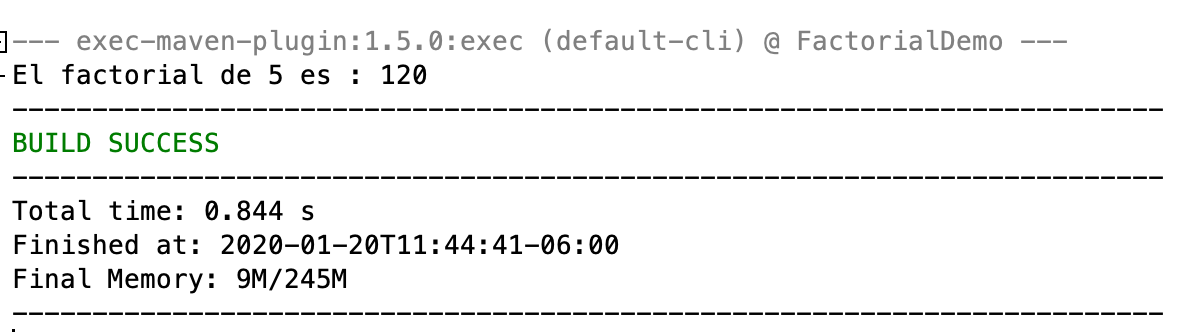
\includegraphics[scale=.54]{factorialIterativo.png}
	\centering \linebreak \linebreak 
	\caption{Factorial Iterativo}
	\label{img:factorialIterativo}
\end{figure} \hfill 
\pagebreak

\subsubsection{\textit{ \color{colorESCOM}{Factorial Resursivo }}}
\lipsum[2-3]

\begin{figure}[H]
	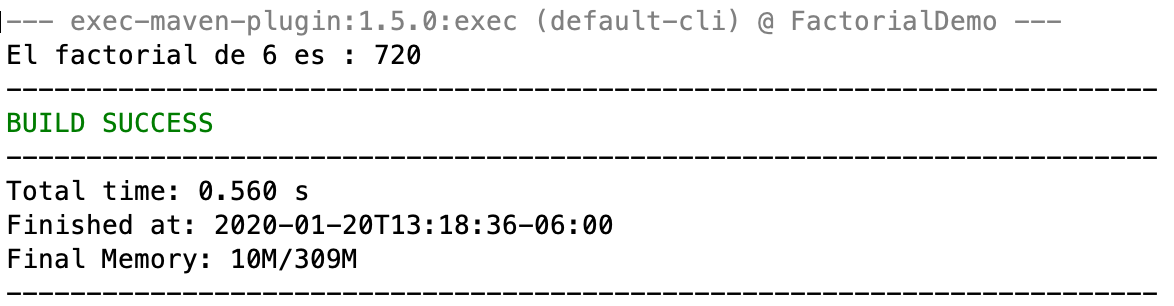
\includegraphics[scale=.54]{factorialRecursivo.png}
	\centering \linebreak \linebreak 
	\caption{Factorial Recursivo}
	\label{img:factorialRecursivo}
\end{figure}  \hfill


\pagebreak


%################################################
\section{\color{colorIPN}{Conclusión}}
\lipsum[2-3]

\begin{table}[htb]
	\centering
	\begin{tabular}{p{2cm} |p{2cm} |p{2cm} |p{3cm}}\hline \hline
		&PP    	& SP   & TP \\ \hline \hline
		Attendance           &  10    & 10 & 10\\ \hline 
		HomeWork           &  20    & 10 & 10\\ \hline 
		Exercises              &  20    & 20 & 20\\ \hline 
		Practices               &  20    & 20 & 25\\ \hline 
		Quiz                      &  20    & 20 & 10\\ \hline 
		Projects                &  10    & 20 & 25  \\ \hline 
		&  100    & 100 & 100\\ \cline{1-2}
		
		\hline \hline
	\end{tabular}
			\caption{Citerios de Evaluacion}
	\label{tabla:Criterios}
\end{table}

\color{colorIPN}{
	\begin{flushright}
		\textit{
			Pedro Pica Piedra
		}
	\end{flushright} \hfill \break
}

\pagebreak

%################################################

\section{\color{colorIPN}{Referencias Bibliográficas}}
\color{colorESCOM}{
	\begin{thebibliography}{10}
		\bibitem[Oracle, 2018]{Oracle}
		Oracle.
		\newblock {\em Web Component Development With Servlet and JSP Technologies}
		\newblock Oracle.
	
		\bibitem[Devlin, 2002]{Devlin}
		Edgar Martinez, Tom McGinn, Eduardo Moranchel, Anjana Shenoy, Michael Williams.
		\newblock {\em Java EE 7: Back-end Server Application Development}
		\newblock Oracle, 2016.
	
		\bibitem[Jendrock, 2014]{Jendrock}
		Eric Jendrock, Ricardo Cervera-Navarro, Ian Evans, Kim Haase, William Markito.
		\newblock {\em Java Platform, Enterprise Edition (Java EE) 8
		The Java EE Tutorial}
		\newblock Oracle, 2017.	
	\end{thebibliography}
}

\end{document}
